\documentclass[12pt,letterpaper,oneside]{book}
\usepackage{astro-thesis}
\usepackage{lipsum}


\begin{document}
	\begin{titlepage}
		\begin{center}
			
\includegraphics[height=4cm]{img/logofisi.png}
			
			\vspace{1cm}
			
			{\fontsize{20}{35}\selectfont \bf Optimización y estandarización del método de mínima entropía para la búsqueda de periodicidades en series temporales astronómicas\par}
			
			\vspace{20mm}
			
			{\large Juan David Aparicio Gutiérrez}
			
			\vspace{10mm}
			
			{\large Director: Dr. José Alejandro García Varela } 
			
			\vspace{15mm}
			
			{\large
				Proyecto Teórico Computacional 
			}
			
			\vspace{5mm}
			
			{\large
				Universidad de los Andes\\
				Facultad de Ciencias, Departmento de Física\\
				Bogotá, Colombia\\ \phantom{} \\
				2026-10
			}
		\end{center}
	\end{titlepage}
    
    
\frontmatter 

\chapter*{Resumen}

\lipsum{3}

%
%\newpage

%\begin{flushright}
	%\textit{
	%	My        \\
	%%%%	Cheesy           \\
	%%%	words
%%	}
%\end{flushright}

%\vspace{2mm}

%\chapter*{Acknowledgements}

%\lipsum{4}

\mainmatter

\tableofcontents

\newpage

\listoffigures
\listoftables
%\listoflistings

\newpage

\visibleintentfalse

\chapter{Estado del arte}
\section{Estrellas binarias y masas estelares}
Esta sección se basa principalmente en el capítulo 10 de \cite{Karttunen2016}. Las estrellas binarias son sistemas de dos estrellas que orbitan de manera conjunta con respecto al centro de masa del sistema. Cuando la diferencia de tamaño entre los dos cuerpos es considerablemente grande, es común que se llame a una la estrella primaria y a la otra, la secundaria. Según lo que se aprecia al observarlas, se pueden definir dos tipos de estrellas binarias: las ópticas y las visuales. Las estrellas binarias ópticas corresponden a aquellas que aparentan ser una sola, mientras que las visuales son aquellas que permiten ver que hay dos componentes al ser observadas. Esto al tener una separación mayor a 0.1 segundos de arco. 

Las estrellas binarias también se clasifican según la separación entre los dos cuerpos. Las distantes presentan una separación de decenas o cientos de unidades astronómicas. Las binarias cercanas tienen una separación de una unidad astronómica hasta el radio de una de las estrellas. Y las binarias de contacto están lo suficientemente cerca como para tocarse. 

Otra clasificación que se utiliza en las estrellas variables depende de cómo se descubren: astrométricas, espectroscópicas y fotométricas o eclipsantes. 

A continuación, ahondaré en ciertos tipos de estrellas variables que resultan de particular interés en este proyecto. 

\subsection{Estrellas Binarias Visuales}
Lo que observamos de binarias visuales consiste en la proyección de la elipse orbital relativa en el plano de nuestro cielo. La forma y posición exactas de la orbita real no se conocen, aunque pueden ser estimadas. Las masas de cada estrella pueden ser determinadas observando sus trayectorias. Cada cuerpo traza una elipse propia alrededor del centro de masa del sistema, de modo que para cada elipse hay una longitud de semieje mayor $a$ entre el centro de la elipse y el punto más alejado de esta. La figura \ref{fig:elipses_visibles}  muestra un diagrama que ilustra este sistema, con $a_1$ y $a_2$ siendo los semiejes mayores de las orbitas de cada estrella, y $A_1$ y $A_2$ las posiciones de cada estrella en un tiempo $A$, $B$ o $C$. Entonces, las masas se relacionan con los semiejes a través de la ecuación \ref{eq:masas_semiejes_binarias_visibles} \cite{Karttunen2016}, donde $m_1$ y $m_2$ son las masas de las estrellas. Así mismo, el semieje mayor de la órbita relativa está dado por la ecuación \ref{eq:semieje_mayor_total} \cite{Karttunen2016}.

\begin{equation}
    \frac{a_1}{a_2} = \frac{m_2}{m_1}
    \label{eq:masas_semiejes_binarias_visibles}
\end{equation}

\begin{equation}
    a=a_1+a_2
    \label{eq:semieje_mayor_total}
\end{equation}

\begin{figure}[h]
	\begin{center}
	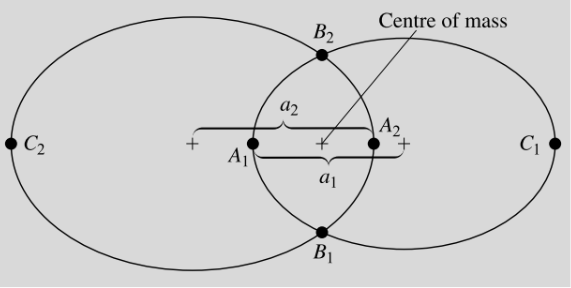
\includegraphics[width=15cm]{img/Fig 10.3 - Karttunen 2016.png}
	\caption{Orbitas de un sistema de estrellas variables que se mueven alrededor del centro de masa. Tomada de \cite{Karttunen2016}.}
    \label{fig:elipses_visibles}
    \end{center}
\end{figure}

\subsection{Estrellas Binarias Astrométricas}
En este tipo de estrellas binarias, solamente se ve un componente, pero su movimiento propio variable indica que debe haber un segundo elemento invisible. Solamente se puede observar la órbita del elemento más brillante, pero si la masa de este es estimada, la masa de la estrella invisible también se puede calcular. 

\subsection{Estrellas Binarias Espectroscópicas}
Estas son descubiertas con base en el espectro que se obtiene del sistema. Se establece que el espectro observado corresponde a un sistema binario por dos razones: o se ven dos conjuntos de líneas espectrales, o el desplazamiento Doppler de las líneas varía de forma periódica. De hecho, en este último caso, el período de variación es equivalente al período orbital de las estrellas.

El desplazamiento por efecto Doppler de una línea espectral es directamente proporcional a la velocidad radial de la estrella. Por lo tanto, cuando una estrella se aleja de nosotros y la otra se acerca, la separación de las líneas espectrales sería más grande. La velocidad observada $v$ se relaciona con la velocidad verdadera $v_0$ a través de la ecuación \ref{eq:velocidades_bin_espectro} \cite{Karttunen2016}. En esta, la inclinación $i$ es el ángulo entre la línea de observación y la normal del plazo de la orbita.

\begin{equation}
    v=v_0 \sin{i}
    \label{eq:velocidades_bin_espectro}
\end{equation}

Ahora, si consideramos que cada estrella se mueve en una órbita circular de radios $a_1$ y $a_2$ con masas $m_1$ y $m_2$, obtenemos la relación mostrada en la ecuación \ref{eq:masas_semiejes_espectro} \cite{Karttunen2016}. La velocidad orbital verdadera está dada por la ecuación \ref{eq:velocidad_orbital_verdadera_espectro}, donde $P$ es el período orbital. Por lo tanto, incorporando las ecuaciones \ref{eq:velocidades_bin_espectro} y \ref{eq:masas_semiejes_espectro} y resolviendo para $a$, se obtiene la ecuación función de masa \ref{eq:funcion_masa_espectro} \cite{Karttunen2016}. El lado izquierdo de esta sería la función de masa. Si una de las dos estrellas es tan tenue que no se pueden observar sus líneas espectrales, entonces solo se observan $P$ y $v_1$. Ni las masas individuales de los componentes ni la masa total del sistema se pueden determinar. En cambio, si las líneas espectrales de ambos participantes se conocen, entonces $v_2$ es conocido también.
 
\begin{equation}
    a_1=\frac{am_2}{m_1+m_2}
    \label{eq:masas_semiejes_espectro}
\end{equation}

\begin{equation}
    v_{0,1}=\frac{2\pi a_1}{P}
    \label{eq:velocidad_orbital_verdadera_espectro}
\end{equation}

\begin{equation}
    \frac{m^3_2 \sin^3{i}}{(m_1+m_2)^2}=\frac{v^3_1P}{2\pi G}
    \label{eq:funcion_masa_espectro}
\end{equation}
   
\subsection{Estrellas Binarias Fotométricas}
Las estrellas binarias fotométricas son sistemas dobles en los que la evidencia observacional principal proviene de variaciones periódicas en el brillo total del sistema. Estas variaciones están asociadas al movimiento orbital de las componentes y se analizan a través de la curva de luz.

En la mayoría de los casos, las binarias fotométricas corresponden a sistemas eclipsantes, donde una estrella pasa frente a la otra desde la línea de visión del observador. Existe también una subclase importante, las variables elipsoidales, en las que no ocurren eclipses propiamente dichos, pero al menos una de las estrellas está deformada por efectos de marea. Debido a esta deformación, el área proyectada y la temperatura superficial efectiva cambian a lo largo de la órbita, produciendo pequeñas variaciones en el brillo observado.

En el caso de las binarias eclipsantes, la inclinación orbital debe ser cercana a $90^\circ$. Esta condición hace que dichas binarias sean especialmente valiosas, ya que son los únicos sistemas espectroscópicos para los cuales la inclinación orbital es conocida, lo que permite determinar de manera única las masas estelares.

La variación temporal del brillo en estos sistemas se denomina \emph{curva de luz}. A partir de la forma de la curva de luz, las binarias eclipsantes se clasifican en tres tipos principales: Algol, $\beta$ lyr\ae y W Ursae Majoris.

\textbf{Estrellas tipo Algol} Las binarias tipo Algol presentan una curva de luz casi constante durante la mayor parte del período orbital, con dos mínimos bien definidos. El mínimo primario es más profundo y ocurre cuando la estrella más brillante es eclipsada por la componente más débil. El mínimo secundario corresponde al eclipse inverso y suele ser menos profundo debido a la diferencia de luminosidades entre las estrellas.

La forma de los mínimos depende de si el eclipse es parcial o total. En un eclipse parcial, el brillo cambia de manera continua, produciendo mínimos suaves. En un eclipse total, una de las estrellas queda completamente oculta durante un intervalo finito, lo que genera un mínimo con fondo plano. Esta característica permite inferir información sobre la inclinación orbital.

La duración de los eclipses está relacionada con la razón entre los radios estelares y el tamaño de la órbita. Si el sistema es además una binaria espectroscópica, el tamaño físico de la órbita puede determinarse, lo que permite obtener las masas y radios estelares sin necesidad de conocer la distancia al sistema.

\textbf{Estrellas tipo $\beta$ lyr\ae} En las binarias tipo $\beta$ lyr\ae, el brillo varía de manera continua a lo largo de todo el período orbital. Esto se debe a que las estrellas están tan próximas que una de ellas se encuentra deformada en una forma elipsoidal. Como resultado, la luminosidad cambia incluso fuera de los eclipses. Estos sistemas pueden interpretarse como binarias eclipsantes con componentes elipsoidales.

En algunos casos, como en el sistema $\beta$ lyr\ae original, una de las estrellas ha sobrepasado su lóbulo de Roche y transfiere masa a su compañera. Este proceso de transferencia introduce características adicionales en la curva de luz.

\textbf{Estrellas tipo W Ursae Majoris} Las binarias tipo W Ursae Majoris presentan mínimos casi idénticos, amplios y redondeados en la curva de luz. Se trata de sistemas muy compactos en los que ambas estrellas llenan sus lóbulos de Roche, formando una binaria de contacto.

\textbf{Efectos adicionales en las curvas de luz} La interpretación de las curvas de luz puede verse complicada por diversos efectos físicos. Entre ellos se incluyen la deformación por fuerzas de marea de las estrellas, el oscurecimiento gravitacional en estrellas elongadas, los efectos de reflexión mutua y los cambios de temperatura asociados a la transferencia de masa.

Debido a estas complejidades, el análisis de binarias fotométricas suele realizarse mediante modelos teóricos detallados. En estos modelos se calcula una curva de luz sintética que se compara con las observaciones, ajustando los parámetros del sistema hasta obtener un acuerdo satisfactorio.

Las estrellas binarias constituyen la principal fuente de masas estelares determinadas con precisión. Las masas de estrellas aisladas se estiman a partir de relaciones masa--luminosidad, las cuales deben calibrarse utilizando observaciones de sistemas binarios \cite{Karttunen2016}.

\section{Sobre el proyecto OGLE}
El artículo \cite{udalski2002bvi} presenta los mapas fotométricos en $V$ e $I$ del bulbo galáctico obtenidos durante la fase OGLE-II del proyecto OGLE. Es un catálogo masivo con fotometría media y astrometría de aproximadamente $3\times10^{7}$ estrellas distribuidas en 49 campos que cubren unos $\sim 11$ deg$^{2}$ en la región central de la Vía Láctea.

Las observaciones fueron realizadas con el telescopio de 1.3 m en Las Campanas, usando un CCD 2048$\times$2048 en modo drift-scan. La mayoría de las imágenes se tomaron en banda $I$ (entre 150 y 570 por campo), mientras que en $V$ se obtuvieron muchas menos (5–18). El seeing mediano fue de aproximadamente $1.25''$, lo cual es importante porque se trata de campos extremadamente densos.

La reducción de datos se hizo con el pipeline estándar de OGLE. Se utilizó DOPHOT en modo de posición fija, tomando como referencia una imagen plantilla con muy buen seeing. La fotometría instrumental se transformó al sistema estándar de Landolt mediante relaciones lineales del tipo
\begin{equation}
V = v - 0.002 (V-I) + \mathrm{const}_{V},
\end{equation}
\begin{equation}
I = i + 0.029 (V-I) + \mathrm{const}_{I},
\end{equation}
\begin{equation}
V-I = 0.969 (v-i) + \mathrm{const}_{V-I}.
\end{equation}

Los residuos típicos respecto a estándares no superan $\sim 0.03$ mag en el rango calibrado ($V-I < 2$). Sin embargo, el artículo discute con cuidado posibles errores sistemáticos para estrellas muy rojas ($V-I > 2$), que son comunes en el bulbo por la alta extinción interestelar. Debido a que el filtro $I$ usado (vidrio RG9) tiene una cola roja más extendida que el estándar, puede introducirse una diferencia sistemática que podría llegar hasta $\sim 0.2$–$0.25$ mag para colores muy extremos. Se modela este efecto usando atmósferas de Kurucz y leyes de extinción estándar.

En cuanto a precisión fotométrica, las comparaciones en regiones de solapamiento entre campos muestran diferencias medias menores a 0.01 mag y dispersión típica $\sim 0.025$ mag. La completitud depende fuertemente de la densidad estelar, pero es alta (mayor al 90\%) hasta $I \approx 17$–18 mag en campos menos congestionados.

Los diagramas color–magnitud ($I$ vs $V-I$) muestran claramente las poblaciones típicas hacia el centro galáctico: secuencia principal del disco (estructura casi vertical azul), rama gigante roja del bulbo con un red clump prominente, y el turn-off del bulbo. También se ve muy fuerte el efecto de la extinción diferencial, que ensancha y desplaza las secuencias dependiendo del campo observado. En campos muy cercanos al centro, la extinción puede ser tan alta que solo se distingue claramente la secuencia principal del disco.

Finalmente, el catálogo se publica electrónicamente y contiene para cada estrella coordenadas ecuatoriales, posiciones en píxeles, magnitudes medias, número de observaciones y dispersión. Aunque el mapa contiene solo magnitudes medias, la dispersión en banda $I$ permite identificar candidatos a estrellas variables. De hecho, el trabajo menciona que ya se había liberado un catálogo preliminar con $\sim 2\times10^{5}$ variables.
	
\chapter{Problema de investigación}
El método de mínima propuesto por \cite{cincotta1995astronomical} tiene ventajas importantes sobre otros métodos basados en Fourier: tiene un respaldo matemático sólido en la teoría de la información y es bastante sencillo de implementar. Sin embargo, su adopción generalizada se limita por dos factores principales. 

\textbf{Arbitrariedad en los parámetros:} como se evidencia en \cite{cubillos2021}, el método requiere definir el tamaño de la grilla de forma arbitraria. En la tesis, estos valores se eligieron de manera empírica y se mantuvieron constantes para todas las estrellas de un mismo tipo. Esto puede que no sea la configuración óptima para cada curva de luz individual y puede afectar la precisión y el número mínimo de puntos que se necesitan para calcular el período.

\textbf{Falta de accesibilidad:} no existe una implementación moderna, bien documentada y fácil de usar en Python. Una librería así, que también tenga criterios de optimización, facilitaría el acceso a un algoritmo potente y permitiría a la comunidad compararlo sistemáticamente con otros métodos como Lomb-Scargle o fnpeaks.

Una mejor selección de la grilla podría tener muchos efectos positivos: reducir el número mínimo de puntos necesarios, mejorar la discriminación de aliases en curvas complejas como las RR Lyr\ae{} y las $\beta$ Lyr\ae, y hacer el método más robusto y menos dependiente de la intuición del usuario.

De este modo, la pregunta de investigación es: ¿cuál es la combinación óptima de parámetros ---tamaño de grilla, rango de períodos y cadencia--- que maximiza la eficiencia y precisión del método de mínima entropía para la determinación de períodos en distintos tipos de estrellas variables, y cómo se puede implementar este método optimizado en una librería de Python de código abierto?

\chapter{Objetivos}
\section{Objetivo general}
Desarrollar y validar una versión optimizada del método de mínima entropía para la búsqueda de períodos, implementada en una librería de Python de código abierto, que determine automáticamente parámetros adecuados según las características de la serie temporal y el tipo de estrella variable.

\section{Objetivos específicos}
\begin{enumerate}
    \item Implementar el algoritmo base de mínima entropía en Python y caracterizar el impacto del tamaño de grilla, el rango de períodos y la cadencia sobre la precisión del período recuperado y el número mínimo de puntos necesarios para una detección exitosa.

    \item Desarrollar un criterio de optimalidad que relacione la morfología de la curva de luz con la configuración de grilla que produce mejores resultados, e implementarlo en un algoritmo que recomiende parámetros iniciales de forma automática.

    \item Construir y documentar una librería de Python que incorpore la lógica de optimización de parámetros y esté lista para su publicación en GitHub y PyPI.

    \item Validar la librería sobre un conjunto de prueba independiente y comparar su rendimiento ---en precisión y tiempo de cómputo--- contra la versión con parámetros fijos, el método de Lomb-Scargle y fnpeaks.
\end{enumerate}

\chapter{Metodología}
\section{Implementación base y barrido de parámetros}
Se implementará el algoritmo de mínima entropía en Python replicando los resultados de \cite{cincotta1995astronomical} y \cite{cubillos2021} como línea base. Sobre un conjunto representativo de estrellas de cada tipo (tomadas de los catálogos OGLE), se realizará un barrido sistemático de tamaños de grilla desde $2\times2$ hasta $15\times15$, combinado con distintos rangos de períodos y cadencias. Para cada configuración se registrará la precisión del período encontrado. Esta precisión se define como el \textit{recovery rate} o tasa de recuperación, en donde se evalúa si el método recupera un múltiplo del período real. 

\section{Desarrollo del criterio de optimalidad}
Con los resultados del barrido se explorará la relación entre la morfología de la curva de luz y la configuración de grilla óptima. Se propondrán y probarán métricas predictivas ---por ejemplo, grillas finas en el eje de magnitud para curvas con variaciones pequeñas, o grillas finas en la fase para sistemas con cambios rápidos como las RR Lyr\ae que permitan recomendar parámetros antes de aplicar el método. El criterio resultante se implementará como un módulo de selección automática de parámetros.

\section{Construcción de la librería}
Se desarrollará el paquete de Python con una API limpia e intuitiva que integre tanto el algoritmo base como la lógica de optimización. Se redactará documentación completa con ejemplos de uso y se preparará el repositorio para su publicación en GitHub y PyPI.

\section{Validación y análisis comparativo}
La librería se evaluará sobre un conjunto de prueba que no haya participado en la fase de desarrollo. Se comparará el rendimiento de la versión optimizada frente a: (i) la versión del método con parámetros arbitrarios fijos, (ii) el método de Lomb-Scargle y (iii) fnpeaks, utilizando como métricas la precisión en el período recuperado, el tiempo de cómputo y el número mínimo de puntos requeridos.

\chapter{Resultados}
\lipsum{20}

\chapter{Conclusiones}
\lipsum{20}

% Bibliography

\nocite{*}%test

\bibliographystyle{aa_url} % style aa.bst
\bibliography{global.bib}

% Appendices

\appendix
%\appendixpage
\noappendicestocpagenum
\addappheadtotoc

%\chapter{Code utilities}
%\lipsum{2}

%\begin{listing}[H]
%	\begin{minted}{c}
%	double eps(double x) {
%	    long i = *(long*) &x;
%	    i++;
%	    double x_next = *(double*) &i;
%	    return x_next - x;
%	}
%	\end{minted}
%	\caption[\texttt{eps} C function]{
%		C code
%	}
%	\label{lst:c-eps}
%\end{listing}

%\lipsum{2}

\chapter{Complementary figures}
\lipsum{20}












\end{document}